\definecolor{keyword}{RGB}{0, 0, 255}
\definecolor{string}{RGB}{255, 0, 0}
\definecolor{comment}{RGB}{0, 128, 0}
\definecolor{number}{RGB}{128, 0, 128}
\definecolor{operator}{RGB}{0, 128, 128}

\lstdefinestyle{graphql}{
    basicstyle=\ttfamily,
    keywordstyle=\color{keyword},
    stringstyle=\color{string},
    commentstyle=\color{comment},
    breaklines=true,
    aboveskip=1em,    % Space above the listing
    belowskip=1em,    % Space below the listing
    morekeywords={query, mutation, subscription, type, interface, fragment, getUsers, getUser, addUser, String, User, Status }, % Add GraphQL keywords
}

\section{Umsetzung}
\subsection{Datenbank-Werkzeuge}
\subsubsection{DynamoDB}
\subsection{API}
\subsubsection{GraphQL}
Der GraphQL-Code erfüllt zwei verschiedene Aufgaben \cite{GraphQLAWSAppSync2024}: Er definiert das Schema der Datenbank: zwar sind in DynamoDB keine Spalten vorgegeben, eine spaltenunabhängige Codierung ist im Rahmen dieses Projekts aber weder semantisch vorteilhaft noch im Rahmen der Praxisarbeit zeitlich realisierbar. Deshalb wird die Tabelle mit den jeweiligen Datentypen vorgegeben:

	\begin{figure}[H]
	\centering
	\begin{minipage}[t]{.7\textwidth} % Breite, z.B. 1\textwidth		
	\caption{Datentypen} % Überschrift
	\begin{lstlisting}[style=graphql]
	type User {
	  email: String!
	  name: String!
	  status: Status
	}
	\end{lstlisting}
	\textit{Eigene Darstellung} % Quelle
	\label{fig:datenTypen}
	\end{minipage}
	\end{figure}
Bezogen auf den Nutzer werden drei Attribute gespeichert: Die email als String, der Name als String und der Status. Dieser ist entweder ``ACTIVE'' oder ``INACTIVE''. Um das zu erreichen muss in GraphQL ein sogenannter ``enum'' erstellt werden. Enums sind Strukturen, die eine Reihe verschiedener Optionen enthalten. Es werden nur Werte akzeptiert, die so auch in der Struktur gespeichert sind (In diesem Fall ACTIVE und INACTIVE). \cite{https://graphql.com/learn/enums/}

	\begin{figure}[H]
	\centering
	\begin{minipage}[t]{.7\textwidth} % Breite, z.B. 1\textwidth		
	\caption{Status} % Überschrift
	\begin{lstlisting}[style=graphql]
	enum Status {
	  ACTIVE
	  INACTIVE
	}
	\end{lstlisting}
	\textit{Eigene Darstellung} % Quelle
	\label{fig:status}
	\end{minipage}
	\end{figure}

Zusätzlich dazu werden in GraphQL die Funktionen der API definiert. Den Anforderungen (s.o.) entsprechend muss es drei Funktionen, eine Mutation und zwei Abfragen geben. Die Abfrage ``GetUsers'' benötigt keine Eingabe, da ohne Selektion alle in der Datenbank enthaltenen Einträge ausgegeben werden. Die Abfrage ``GetUser'' hingegen benötigt die E-Mail als Filterparameter, und die Mutation AddUser braucht alle 3 Informationen über den Nutzer. Das muss in der Definition berücksichtigt werden:

	\begin{figure}[H]
	\centering
	\begin{minipage}[t]{.7\textwidth} % Breite, z.B. 1\textwidth		
	\caption{Query und Mutation} % Überschrift
	\begin{lstlisting}[style=graphql]
	type Query {
	  getUsers: [User]
	  getUser(email: String!): User
	}
	
	type Mutation {
	  addUser(email: String!, name: String,! status: Status): User
	}
	\end{lstlisting}
	\textit{Eigene Darstellung} % Quelle
	\label{fig:queryAndMutation}
	\end{minipage}
	\end{figure}


\subsubsection{API-Methoden}
Für jede API-Methode existiert eine JavaScript-Datei. Die Methoden unterscheiden sich aufgrund ihrer unterschiedlichen Anforderungen.
\paragraph{Bibliothek}
Um Daten aus der Tabelle mit JavaScript zu editieren, wird eine Bibliothek verwendet, in der verschiedene Standard-Operationen enthalten sind, die auf einer DynamoDB-Tabelle ausgefürt werden können. Auf Basis dieser Bibliothek sind dann alle Methoden aufgebaut. Die Bibliothek wird in allen Dateien unter dem gleichen Alias importiert, weshalb der Import kein Teil der Code-Snippets für die Methoden ist, und stattdessen im Folgenden beispielhaft isoliert dargestellt wird. Der Name, mit der die Bilbiothek referenziert wird, ist ``ddb'':\newline
	\begin{figure}[H]
	\centering
	\begin{minipage}[t]{.7\textwidth} % Breite, z.B. 1\textwidth		
	\caption{Import der Bibliothek} % Überschrift
	\begin{minted}[breaklines=true]{javascript}
	import * as ddb from '@aws-appsync/utils/dynamodb'
	\end{minted}
	
	\textit{Eigene Darstellung} % Quelle
	\label{fig:bibliothekImport}
	\end{minipage}
	\end{figure}
\paragraph{Aufbau der Dateien}
Da in allen JavaScript-Dateien jeweils eine API-Funktion definiert wird, ist der grundlegende Aufbau identisch. Die Dateien unterscheiden sich lediglich durch den Inhalt der Methode selbst. 
Auf den oben beschriebenen Import der Bibliothek folgend wird die Funktion ``request'' definiert. Die Funktion dient der Behandlung der Anfrage, das Resultat der Methode wird als ``result'' in der Kontext-Variable gespeichert. Die Kontext-Variable wird als Input-Parameter in die Methode gegeben und beinhaltet alle relevanten Informationen rund um die Anfrage. Das Resultat hat keinen vorgegbenen Datentyp:\newline
	\begin{figure}[H]
	\centering
	\begin{minipage}[t]{.7\textwidth} % Breite, z.B. 1\textwidth		
	\caption{Methode Request} % Überschrift
	\begin{minted}[breaklines=true]{javascript}
	export function request(ctx) {
	  //handle the request
	  //return the result
	}
	\end{minted}
	
	\textit{Eigene Darstellung} % Quelle
	\label{fig:requestMethode}
	\end{minipage}
	\end{figure}

Nachdem die Abfrage durch die Request-Methode behandelt wurde, muss auch die Ausgabe behandelt werden. Das geschieht über die Funktion ``response''. Sollte keine weitere Mutation des Resultats nötig sein, sieht diese Methode folgendermaßen aus:\newline
	\begin{figure}[H]
	\centering
	\begin{minipage}[t]{.7\textwidth} % Breite, z.B. 1\textwidth		
	\caption{Methode Response} % Überschrift
	\begin{minted}[breaklines=true]{javascript}
	export const response = (ctx) => ctx.result;
	\end{minted}

	\textit{Eigene Darstellung} % Quelle
	\label{fig:responseMethode}
	\end{minipage}
	\end{figure}
Der Eingabe-Parameter für die Methode ist ctx, also die Kontext-Variable. Ausgegeben wird ctx.result, die Variable in der das Resultat gespeichert wird. Ist ctx.result leer, so wird ``undefined'' zurückgegeben. Die Methode ist also äquivalent zu der Folgenden:\newline
	\begin{figure}[H]
	\centering
	\begin{minipage}[t]{.7\textwidth} % Breite, z.B. 1\textwidth		
	\caption{Alternative Methode Response} % Überschrift
	\begin{minted}[breaklines=true]{javascript}
	export const response = (ctx) => {
	    if (ctx != null) return ctx.result;
	    else return undefined;
	};
	\end{minted}

	\textit{Eigene Darstellung} % Quelle
	\label{fig:alternativeResponseMethode}
	\end{minipage}
	\end{figure}\newpage
	\subsubsection{GetUser}
	
Aus den Anforderungen an diese Methode geht hervor, dass zu den Eingabe-Parametern die email gehören muss, damit nach dieser gefiltert werden kann. Zusätzlich muss noch die Möglichkeit geboten werden, bis zu drei weitere Variablen mitzugeben. Diese stellen dann die Felder dar, die von der API zurückgegeben werden. Für die Ausgabe muss definiert werden, welche Operation ausgeführt wird. Die Antwort ist dann die Rückgabe der Abfrage mit dem Filterparameter:\newline

	\begin{figure}[H]
	\centering
	\begin{minipage}[t]{.7\textwidth} % Breite, z.B. 1\textwidth		
	\caption{Methoden GetUser} % Überschrift
	\begin{minted}[breaklines=true]{javascript}
	export function request(ctx) {
	  return ddb.get({ key: { email: ctx.args.email } });
	}
	
	export const response = (ctx) => ctx.result;
	
	\end{minted}
	
	\textit{Eigene Darstellung} % Quelle
	\label{fig:getUserMethoden}
	\end{minipage}
	\end{figure}
Für die Abfrage wird die Methode ddb.get() verwendet, welche die entsprechend passenden Einträge für einen gegebenen Schlüsselparameter liefert, sofern diese vorhanden sind.
\paragraph{GetUsers}
Aus den Anforderungen an diese Methode geht hervor, dass als Eingabe-Parameter nur die Möglichkeit bestehen muss, die auszugebenden Felder auszuwählen. Für die Ausgabe muss definiert werden, welche Operation ausgeführt wird, \newpage Die Antwort ist dann die Rückgabe der Abfrage:\newline
	\begin{figure}[H]
	\centering
	\begin{minipage}[t]{.7\textwidth} % Breite, z.B. 1\textwidth		
	\caption{Methoden GetUsers} % Überschrift
	\begin{minted}[breaklines=true]{javascript}
	export function request(ctx) {
	  return { operation: 'Scan' };
	}
	
	export const response = (ctx) => ctx.result.items;
	
	\end{minted}
	
	\textit{Eigene Darstellung} % Quelle
	\label{fig:getUsersMethoden}
	\end{minipage}
	\end{figure}
Aufgrund eines Fehlers mit der Methode ddb.scan() wird hier die Bibliothek nicht eingesetzt. Stattdessen wird die Scan-Operation manuell aufgerufen, und das Ergebnis dieser zurückgegeben. Die Antwort wird dann aus allen Items der ctx-result-Variable gebildet.
\paragraph {AddUser}
Aus den Anforderungen an diese Methode geht hervor, dass als Eingabe-Parameter zumindest die email, also der Schlüssel der Tabelle, gegeben sein muss. Dazu muss die Möglichkeit bestehen, Inhalt für alle anderen Spalten mitzugeben, und Spalten zur Ausgabe auszuwählen. Die Ausgabe bei dieser Mutation ist das durch die Methode selbst hinzugefügte Element:
	\begin{figure}[H]
	\centering
	\begin{minipage}[t]{.7\textwidth} % Breite, z.B. 1\textwidth		
	\caption{Methoden AddUser} % Überschrift
	\begin{minted}[breaklines=true]{javascript}
	export function request(ctx) {
	  const { email, ...values} = ctx.args
	  return {
	    operation: 'PutItem',
	    key: util.dynamodb.toMapValues({email}),
	    attributeValues: util.dynamodb.toMapValues(values),
	  };
	}
	export const response = (ctx) => ctx.result;
	\end{minted}
	
	\textit{Eigene Darstellung} % Quelle
	\label{fig:addUserMethoden}
	\end{minipage}
	\end{figure}
Zuerst werden hier die Argumente extrahiert, da diese gesondert genutzt werden. Dafür wird ctx.args, die Variable in der alle Argumente gespeichert sind, auf zwei Variablen verteilt. Das erste Argument (in diesem Fall die email als Schlüssel) wird auf die Variable email übertragen, alle weiteren Argumente auf die Liste values. Danach wird die Operation definiert, hier ``PutItem'', also das Hinzufügen eines Elements, woraufhin die Schlüsselspalte und die anderen Spalten auf die vorher gespeicherten Variablen gesetzt werden. Die Response-Methode ist identisch zu der, die in GetUser verwendet wurde.

\subsubsection{Lambda}
Im Rahmen der Lambda-Funktionen werden drei verschiedene Dateien verwendet. In der Datei ``shared.py'' sind die Methoden hinterlegt, die für alle Funktionen relevant sind. Die Dateien ``success.py'' und ``error.py'' beinhalten jeweils eine Lambda-Funktion, wobei erstere eine korrekte, und zweitere eine fehlerhafte Anfrage simuliert. 
\paragraph{Geteilte Methoden}
Für die Funktionen werden drei verschiedene unterstützende Methoden benötigt (in diesem speziellen Anwendungsfall, diese Zahl ist nicht unbedingt auf andere Projekte übertragbar). Mit einer Methode wird die Instanz eines sogenannten ``logger''s verteilt. Ein logger ist dafür zuständig, Nachrichten über die Ausführung eines Programms auszugeben:\newline
	\begin{figure}[H]
	\centering
	\begin{minipage}[t]{.7\textwidth} % Breite, z.B. 1\textwidth		
	\caption{GetLogger-Methode} % Überschrift
	\begin{minted}[breaklines=true]{python}
	def get_logger(level: int = logging.INFO):
	    logger = logging.getLogger()
	    logger.setLevel(level)
	    return logger
	\end{minted}
	
	\textit{Eigene Darstellung} % Quelle
	\label{fig:getLoggerMethode}
	\end{minipage}
	\end{figure}
Eine weitere Methode ist dafür zuständig, das API-Secret zu generieren, mit welchem sich die Methoden authentifizieren:\newline
	\begin{figure}[H]
	\centering
	\begin{minipage}[t]{.7\textwidth} % Breite, z.B. 1\textwidth		
	\caption{GetSecret-Methode} % Überschrift
	\begin{minted}[breaklines=true]{python}
	def get_secret(secret_id: str) -> str:
	    response = sm_client.get_secret_value(SecretId=secret_id)
	    return response["SecretString"]
	\end{minted}
	
	\textit{Eigene Darstellung} % Quelle
	\label{fig:getSecretMethode}
	\end{minipage}
	\end{figure}
Die letzte Methode ist dafür zuständig die Query auszuführen, die in den beiden anderen Dateien definiert wird. Als Eingabe-Parameter werden die URL der angesprochenen Schnittstelle, der API-Key und die query erwartet:\newline
	\begin{figure}[H]
	\centering
	\begin{minipage}[t]{.7\textwidth} % Breite, z.B. 1\textwidth		
	\caption{Query-Methode} % Überschrift
	\begin{minted}[breaklines=true]{python}
	def query(url: str, key: str, query: str):
	\end{minted}
	
	\textit{Eigene Darstellung} % Quelle
	\label{fig:queryMethode}
	\end{minipage}
	\end{figure}
Die Bearbeitung ist in mehrere Schritte gegliedert:\newline
1. Definition der query:\newline
	\begin{figure}[H]
	\centering
	\begin{minipage}[t]{.7\textwidth} % Breite, z.B. 1\textwidth		
	\caption{Definition der Query} % Überschrift
	\begin{minted}[breaklines=true]{python}
	data = json.dumps({"query": query}).encode()
	\end{minted}
	
	\textit{Eigene Darstellung} % Quelle
	\label{fig:queryDefinition}
	\end{minipage}
	\end{figure}
2. Formierung des requests, indem das Request selbst mit Methode und URL und der Header mit Content-Type und API-Key definiert werden:\newline
	\begin{figure}[H]
	\centering
	\begin{minipage}[t]{.7\textwidth} % Breite, z.B. 1\textwidth		
	\caption{Formierung des Requests} % Überschrift
	\begin{minted}[breaklines=true]{python}
	req = request.Request(url, method="POST")
	    req.add_header("x-api-key", key)
	    req.add_header("Content-Type", "application/graphql")
	\end{minted}
	
	\textit{Eigene Darstellung} % Quelle
	\label{fig:requestFormierung}
	\end{minipage}
	\end{figure}
3. Durchführung der Anfrage und Rückgabe der Antwort:\newline
	\begin{figure}[H]
	\centering
	\begin{minipage}[t]{.7\textwidth} % Breite, z.B. 1\textwidth		
	\caption{Durchführung der Anfrage} % Überschrift
	\begin{minted}[breaklines=true]{python}
	response = request.urlopen(req, data=data)
	return json.loads(response.read())
	\end{minted}
	
	\textit{Eigene Darstellung} % Quelle
	\label{fig:anfrageDurchführung}
	\end{minipage}
	\end{figure}
\paragraph{Simulation der fehlerhaften Abfrage}
Basis der fehlerhaften Anfrage ist eine fehlerhafte Query. Diese sieht folgendermaßen aus:\newline
	\begin{figure}[H]
	\centering
	\begin{minipage}[t]{.7\textwidth} % Breite, z.B. 1\textwidth		
	\caption{Fehlerhafte Query} % Überschrift
	\begin{minted}[breaklines=true]{python}
	QUERY = """
	query MyQuery {
	  getUsers {
	    email
	    name
	    stat
	  }
	}
	"""
	\end{minted}
	
	\textit{Eigene Darstellung} % Quelle
	\label{fig:fehlerhafteQuery}
	\end{minipage}
	\end{figure}
Das Feld ``stat'' existiert nicht, weshalb hier in der Ausführung ein Fehler ausgeworfen wird. 
\newline
Zusätzlich beinhaltet die Datei eine Methode, mit der die Query behandelt wird. Diese teilt sich folgendermaßen auf:\newline
1. Generieren des API-Keys mithilfe der get secret-Methode aus ``shared.py'':\newline
	\begin{figure}[H]
	\centering
	\begin{minipage}[t]{.7\textwidth} % Breite, z.B. 1\textwidth		
	\caption{Generieren des API-Keys} % Überschrift
	\begin{minted}[breaklines=true]{python}
	key = get_secret(os.environ["API_KEY_SECRET_ID"])
	\end{minted}
	
	\textit{Eigene Darstellung} % Quelle
	\label{fig:apiKeyGenerierung}
	\end{minipage}
	\end{figure}
2. Ausführen der Query über die Methode aus  ``shared.py'':\newline
	\begin{figure}[H]
	\centering
	\begin{minipage}[t]{.7\textwidth} % Breite, z.B. 1\textwidth		
	\caption{Ausführen der Query} % Überschrift
	\begin{minted}[breaklines=true]{python}
	result = query(os.environ["API_URL"], key, QUERY)
	\end{minted}
	
	\textit{Eigene Darstellung} % Quelle
	\label{fig:queryAusführung}
	\end{minipage}
	\end{figure}
3. Generieren des loggers mithilfe der Methode aus ``shared.py'' und Dokumentation des Fehlers:\newline
	\begin{figure}[H]
	\centering
	\begin{minipage}[t]{.7\textwidth} % Breite, z.B. 1\textwidth		
	\caption{Generieren des Loggers} % Überschrift
	\begin{minted}[breaklines=true]{python}
	get_logger().error(result)
	\end{minted}
	
	\textit{Eigene Darstellung} % Quelle
	\label{fig:loggerGenerierung}
	\end{minipage}
	\end{figure}
4. Rückgabe des Felds ``errors'' aus dem Resultat:\newline
	\begin{figure}[H]
	\centering
	\begin{minipage}[t]{.7\textwidth} % Breite, z.B. 1\textwidth		
	\caption{Rückgabe des Felds ``errors''} % Überschrift
	\begin{minted}[breaklines=true]{python}
	return result["errors"]
	\end{minted}
	
	\textit{Eigene Darstellung} % Quelle
	\label{fig:errorFeldRückgabe}
	\end{minipage}
	\end{figure}
\paragraph{Simulation der erfolgreichen Abfrage}
Basis der erfolgreichen Abfrage ist eine korrekte Query. Diese sieht folgendermaßen aus:\newline
	\begin{figure}[H]
	\centering
	\begin{minipage}[t]{.7\textwidth} % Breite, z.B. 1\textwidth		
	\caption{Korrekte Query} % Überschrift
	\begin{minted}[breaklines=true]{python}
	QUERY = """
	query MyQuery {
	  getUsers {
	    email
	    name
	    status
	  }
	}
	"""
	\end{minted}
	
	\textit{Eigene Darstellung} % Quelle
	\label{fig:korrekteQuery}
	\end{minipage}
	\end{figure}
Genau wie die Simulation der fehlerhaften Abfrage wird die Query auch hier in einer seperaten Methode behandelt. Diese ist bis auf die Rückgabe identisch. Zurückgegeben wird nicht der Fehler sondern das korrekte Resultat:\newline
	\begin{figure}[H]
	\centering
	\begin{minipage}[t]{.7\textwidth} % Breite, z.B. 1\textwidth		
	\caption{Rückgabe des korrekten Resultats} % Überschrift
	\begin{minted}[breaklines=true]{python}
	return result["data"]["getUsers"]
	\end{minted}
	
	\textit{Eigene Darstellung} % Quelle
	\label{fig:resultatsRückgabe}
	\end{minipage}
	\end{figure}
\subsection{AWS-Infrastruktur}
\subsubsection{Terraform}
Die Basis der in Terraform deifnierten Infrastruktur ist die Verbindung mit der Datenbank und die Definition der zu verwendenden Rollen für die jeweiligen Abfragen. 
\paragraph{Definition der Tabelle}
Zuerst wird dafür eine Resource erstellt, in welcher die von Terraform angeforderten Informationen über die Datenbank angegeben werden \newline \cite{TerraformBestPractices2024}. Dazu gehören der Name der Datenbank, der Zahlungsmodus und der Datenbankschlüssel. Beim Zahlungsmodus unterscheidet AWS zwischen ``provisioned'' und ``pay per request''. Bei unvorhersehbaren Anfragefrequenzen empfiehlt AWS ``pay per request'', weshalb dieses auch hier verwendet wird: Da die Umsetzung auf  dem Testsystem stattfindet, ist nicht von regelmäßiger Nutzung auszugehen. Der Name der Datenbank ist ``users-db'' und der Datenbankschlüssel ist die E-Mail. Mit diesen Informationen kann nun die Ressource erstellt werden:

	\begin{figure}[H]
	\centering
	\begin{minipage}[t]{.7\textwidth} % Breite, z.B. 1\textwidth		
	\caption{Definition der Tabelle} % Überschrift
	\begin{minted}[breaklines=true]{terraform}
	resource "aws_dynamodb_table" "user" {
	  name         = "user-db"
	  billing_mode = "PAY_PER_REQUEST"
	  hash_key     = "email"
	
	  attribute {
	    name = "email"
	    type = "S"
	  }
	}
	
	\end{minted}
	
	\textit{Eigene Darstellung} % Quelle
	\label{fig:tabellenDefinition}
	\end{minipage}
	\end{figure}
\paragraph{Definition der Berechtigungen}
Da die API zwei verschiedene Methoden-Typen anbietet, die jeweils verschiedene Zugriffslevel benötigen, müssen auch zwei verschiedene Zugriffspolitiken aufgesetzt werden. Für Queries muss die API Daten aus der Tabelle lesen können, und für die Mutation die Tabelle editieren. Die beiden Zugriffsberechtigungen sind vom Aufbau her gleich, weshalb im Folgenden nur zur Veranschaulichung der Schreib-Zugriff beschrieben wird. Die Basis bildet hier ein ``IAM policy document''. Dieses JSON-Dokument enthält Informationen, ohne die der Zugriff nicht gewährt werden kann, und bildet somit die Quelle des Zugriffs. Zusätzlich zu dieser Quelle müssen manuell die Aktionen definiert werden, die mit dieser Rolle verbunden sein sollen, und es muss eine Identifikationsnummer für die Rolle vergeben werden. Diese Informationen werden als Datenobjekt abgespeichert, und können dann von der API zur Authorisierung verwendet werden:
\newline
\newline
	\begin{figure}[H]
	\centering
	\begin{minipage}[t]{.7\textwidth} % Breite, z.B. 1\textwidth		
	\caption{Definition der Berechtigungen} % Überschrift
	\begin{minted}[breaklines=true]{terraform}
	data "aws_iam_policy_document" "user_table_write" {
	  source_policy_documents = [data.aws_iam_policy_document.user_table_read.json]
	
	  statement {
	    sid = "WriteItems"
	    actions = [
	      "dynamodb:PutItem",
	      "dynamodb:UpdateItem",
	      "dynamodb:DeleteItem",
	    ]
	    resources = [aws_dynamodb_table.user.arn]
	  }
	}
	
	\end{minted}
	
	\textit{Eigene Darstellung} % Quelle
	\label{fig:berechtigungsDefinition}
	\end{minipage}
	\end{figure}
\paragraph{Definition der Funktions-Resolver}
Für jede Funktion der API muss in Terraform ein sogenannter Resolver angelegt werden. In einem Resolver sind Informationen über die Methode hinterlegt, die ausgeführt werden soll. Enthalten muss ein Resolver den Typ der Funktion, die Idenfikationsnummer der API, die Datengrundlage, den Namen der Funktion, die Art der Funktion, und die Datei, in der die Methode beschrieben wird. Im Rahmen dieser Praxisarbeit sind die Methoden in Javascript definiert\footnote{Die Sprache hat keinen Einfluss auf die Funktionsweise, die Entscheidung beruht ausschließlich auf der Präferenz der Entwickler}. Zuletzt muss noch die Runtime der Sprache, in der die Methoden verfasst sind, definiert werden, damit die Methoden ausgeführt werden können. Der Resolver wird dann als Resource abgespeichert. Beispielhaft ist hier die Methode AddUser dargestellt:

	\begin{figure}[H]
	\centering
	\begin{minipage}[t]{.7\textwidth} % Breite, z.B. 1\textwidth		
	\caption{Definition der Funktions-Resolver} % Überschrift
	\begin{minted}[breaklines=true]{terraform}
	resource "aws_appsync_resolver" "add_user" {
	  type        = "Mutation"
	  api_id      = aws_appsync_graphql_api.user.id
	  data_source = aws_appsync_datasource.user_table.name
	  field       = "addUser"
	  kind        = "UNIT"
	  code        = file("${path.module}/templates/addUser.js")
	
	  runtime {
	    name            = "APPSYNC_JS"
	    runtime_version = "1.0.0"
	  }
	}
	
	\end{minted}
	
	\textit{Eigene Darstellung} % Quelle
	\label{fig:resolverDefinition}
	\end{minipage}
	\end{figure}
\paragraph{Aktivierung des Cloud-Watch-Loggings}
Um das Sammeln von Daten in CloudWatch zu aktivieren, muss eine Methode in Terraform auf die entsprechende Policy referenzieren
\newline
\newline
	\begin{figure}[H]
	\centering
	\begin{minipage}[t]{.7\textwidth} % Breite, z.B. 1\textwidth		
	\caption{Aktivierung des Cloud-Watch-Loggings} % Überschrift
	\begin{minted}[breaklines=true]{terraform}
	resource "aws_iam_role_policy_attachment" "logging" {
	  policy_arn = "arn:aws:iam::aws:policy/service-role/AWSAppSyncPushToCloudWatchLogs"
	  role           = aws_iam_role.logging.name
	}
	\end{minted}
	
	\textit{Eigene Darstellung} % Quelle
	\label{fig:loggingAktivierung}
	\end{minipage}
	\end{figure}

\subsubsection{AWS-Datadog-Integration}
Die praktische Umsetzung der Integration beschränkt sich auf die Eingabe von Daten in den Benutzeroberflächen von DataDog und AWS.
\paragraph{DataDog}
Zuerst muss in DataDog ein neuer AWS-Account als Integration hinzugefügt werden. Dabei werden dem Nutzer vier Anpassungsoptionen gegeben:\newline
1. AWS-Region\newline
In diesem Fall, da die Auftraggebende Abteilung auf diesem Server beheimatet ist, ist die Region ``eu-central-1''\newline
2. API Key\newline
Lässt der Nutzer hier das Feld unverändert, generiert DataDog automatisch einen API-Key. Für dieses Projekt wurde bereits im Vorfeld ein API-Key angelegt, der deshalb hier ausgewählt wird.\newline
3. AWS Logs senden\newline
Damit die im vorigen Kapitel aufgesetzten Lambda-Funktionen einen Nutzen haben, sollte diese Option aktiviert sein.\newline
4. Cloud Security Verwaltung anschalten\newline
Im Rahmen dieser Praxisarbeit ist Sicherheit nicht ausschlaggebend, da keine schützenswerten Daten behandelt werden. Die Kosten für Sicherheit werden dementsprechend gespart und diese Option bleibt deaktiviert.\newline
\newline
Nachdem die Felder ausgefüllt wurden, kann das Template erstellt werden. Damit ist der in DataDog zu absolvierende Teil abgeschlossen. \newline
\paragraph{AWS}
Mit der Fertigstellung des Templates in DataDog wird der Nutzer automatisch in die Applikation ``CloudFormation'' weitergeleitet. Dort kann dann mit dem API-Key aus DataDog und einem App-Key, welcher ebenfalls in DataDog generiert wird, ein Stack erstellt werden. Damit ist die Verbindung abgeschlossen und Daten können zwischen AWS und DataDog fließen.

\subsection{Monitoring}
\subsubsection{DataDog}
Aus den Anforderungen gehen drei verschiedene zu implementierende Module hervor. Das erste ist ein Zeitstrahl, mit dem die Response time im zeitlichen Kontext dargestellt werden kann.  Das andere ist ein Diagramm, durch welches eine Relation zwischen erfolgreichen und nicht erfolgreichen Abfragen hergestellt werden kann. Hier bietet sich ein Tortendiagramm an, ein Balkendiagramm, Strahlendiagramm oder sogar ein Zeitstrahl für Tendenzen wären auch denkbar. Die Auswahl basiert hier nicht darauf, welches Diagramm am besten für den Nutzungsfall geeignet ist. Diese Entscheidung ist auch von Nutzerpräferenz abhängig, und kann aufgrund des frühen Entwicklungsstadiums noch nicht miteinbezogen werden kann.
\paragraph{Zeitstrahl}
Für den Zeitstrahl wird die Metrik ``aws.appsync.latency'' verwendet. Ein Strahl stellt dabei die exakte Response time zu einem bestimmten Zeitpunkt dar, während der andere die zugehörige Trendlinie bildet, die das Visualisieren von Trends vereinfachen soll:\newline

	\begin{figure}[H]
	\centering
	\begin{minipage}[t]{.7\textwidth} % Breite, z.B. 1\textwidth		
	\caption{Zeitstrahl; Einstellungen} % Überschrift
	
	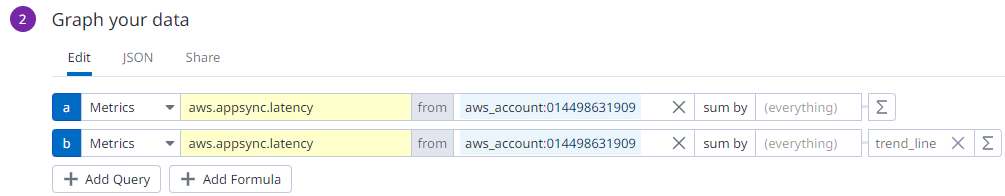
\includegraphics[width = 15cm,keepaspectratio]{graphOneSettings}\newline
	\textit{Eigene Darstellung} % Quelle
	\label{fig:zeitStrahlEinstellungen}
	\end{minipage}
	\end{figure}
	
	Hier ein beispielhafter Ausschnitt des Graphen:
	
	\begin{figure}[H]
	\centering
	\begin{minipage}[t]{.7\textwidth} % Breite, z.B. 1\textwidth		
	\caption{Zeitstrahl} % Überschrift
	
	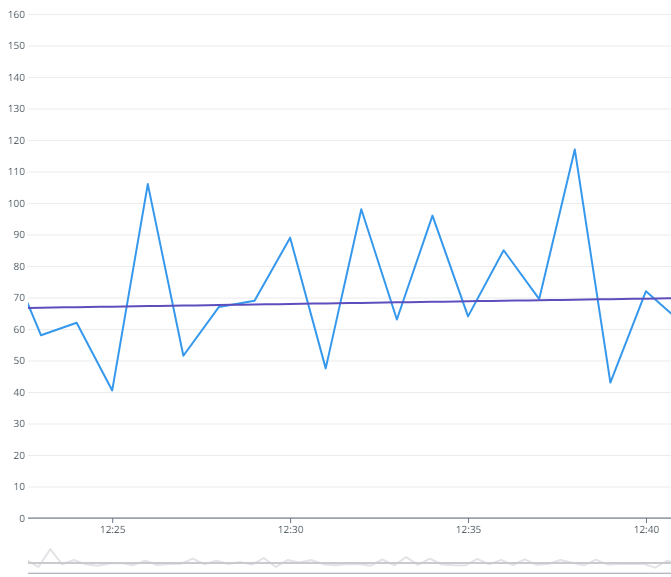
\includegraphics[width = 8cm,keepaspectratio]{graphOneItself} \newline
	
	\textit{Eigene Darstellung} % Quelle
	\label{fig:zeitstrahl}
	\end{minipage}
	\end{figure}
 
\paragraph{Tortendiagramm}
Zur Umsetzung des Tortendiagramms müssen die Filter so gewählt werden, dass mit einer einzigen OR-Abfrage informative logs von fehlerhaften und erfolgreichen Abfragen (im Folgenden Antworten) unterschieden werden können. Unter anderem unterscheiden sich die beiden JSONs der Antwort-Logs von den informativen logs darin, dass in Informativen Logs kein Event existiert. Die variable ``evt.name'' existiert nur in Antwort-Logs. Der Filter wird also folgendermaßen aufgebaut: \newline
\begin{figure}[H]
\centering
	\begin{minipage}[t]{.7\textwidth} % Breite, z.B. 1\textwidth		
	\caption{Tortendiagramm Filter} % Überschrift
	
	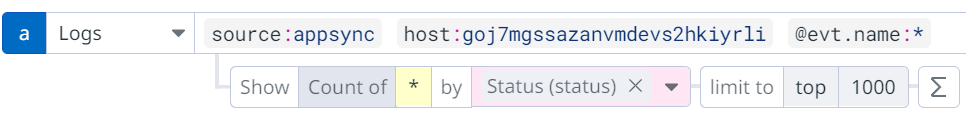
\includegraphics[width = 8cm,keepaspectratio]{pieChartFilter} \newline
	
	\textit{Eigene Darstellung} % Quelle
	\label{fig:pieChartFilter}
	\end{minipage}
	\end{figure}
Es sollen nur Logs der API, an der dieses Projekt durchgeführt wird, und von AppSync gesendet wurden in dieses Tortendiagram einfließen. Das stellen die ersten beiden Filter sicher. Danach wird ein sogenannter Wildcard-Filter auf das Feld ``evt.name'' angewendet. Das bedeutet, dass alle Logs in dieses Diagramm einfließen, die irgendeinen Wert für dieses Feld haben. Da das Feld nur für Antwort-Logs existiert, werden dadurch alle informativen Logs herausgefiltert, und das gewünschte Diagramm erreicht:\newline

	\begin{figure}[H]
	\centering
	\begin{minipage}[t]{.7\textwidth} % Breite, z.B. 1\textwidth		
	\caption{Tortendiagramm} % Überschrift
	
	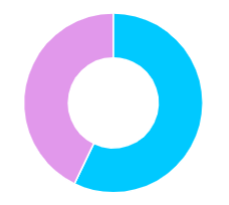
\includegraphics[width = 8cm,keepaspectratio]{pieChart} \newline
	
	\textit{Eigene Darstellung} % Quelle
	\label{fig:pieChart}
	\end{minipage}
	\end{figure}
\subsubsection{CloudWatch}
Aus dem DataDog-Dashboard lässt sich, sollte der Bedarf bestehen, zu jedem Log eines Fehlers der jeweilige logStream herauslesen:\newline

	\begin{figure}[H]
	\centering
	\begin{minipage}[t]{.7\textwidth} % Breite, z.B. 1\textwidth		
	\caption{LogStream} % Überschrift
	
	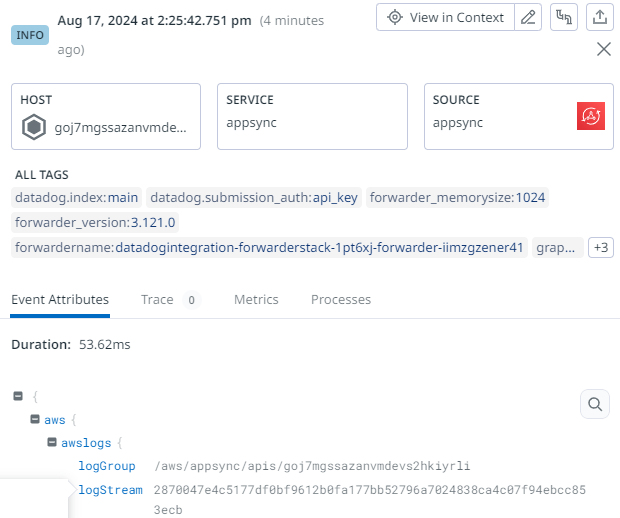
\includegraphics[width = 8cm,keepaspectratio]{logStream} \newline
	
	\textit{Eigene Darstellung} % Quelle
	\label{fig:logStream}
	\end{minipage}
	\end{figure}
 
Mit dieser Identifikationsnummer kann dann auf den LogStream in CloudWatch zugegriffen werden, in welchem alle Informationen zu dem Fehler aufzufinden sind. Das ist möglich, indem innerhalb der LogStream-Sammlung der API mithilfe der Identifikationsnummer gefiltert wird:\newline

	\begin{figure}[H]
	\centering
	\begin{minipage}[t]{.7\textwidth} % Breite, z.B. 1\textwidth		
	\caption{Filter für den LogStream} % Überschrift
	
	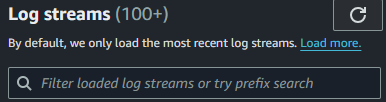
\includegraphics[width = 8cm,keepaspectratio]{logStreamFilter} \newline
	
	\textit{Eigene Darstellung} % Quelle
	\label{fig:logStreamFilter}
	\end{minipage}
	\end{figure}
 
Hier ein beispielhafter Ausschnitt aus den Logs:
	\begin{figure}[H]
	\centering
	\begin{minipage}[t]{.7\textwidth} % Breite, z.B. 1\textwidth		
	\caption{LogStream Beispiel} % Überschrift
	
	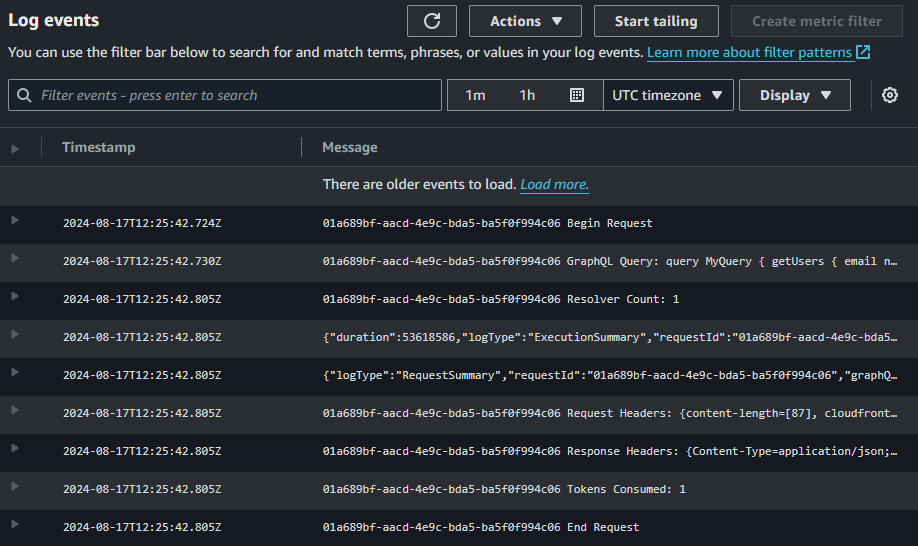
\includegraphics[width = 8cm,keepaspectratio]{logStreamExample} \newline
	
	\textit{Eigene Darstellung} % Quelle
	\label{fig:logStreamBeispiel}
	\end{minipage}
	\end{figure}
 
Durch die Informationen, die aus diesen Logs hervorgehen (Fehlertyp, Stelle im Code/in der Abfrage), ist das Debuggen der Fehler erleichtert. 